\clearpage
\section{Secondary vertices \label{sec:secondaryvertex}}
Secondary vertex reconstruction is performed using the “Adaptive Vertex Finder” \cite{bib:AVF}, which performs a fully inclusive vertex search in a list of given tracks. The approach is to fit a vertex from all tracks
and iteratively repeat the fit with tracks that were not compatible with the vertices obtained
in previous iterations. This procedure is repeated until the list of tracks is exhausted or the
vertex fit fails. The “Adaptive Vertex Fitter” is used for the actual vertex fit performed at each
iteration. Since all candidate tracks are passed to it at once, it is able to intrinsically identify and
deal with outliers to allow for the fit to converge. It therefore applies an iterative procedure, by which outlier tracks are increasingly downweighted. This is done until the fit converges and
thus only compatible tracks, which have sizable weights, remain.

The parameters used are primcut = 1.8 and seccut = 6.0. Both denote the track-vertex compatibility
cutoff parameter used for the first and all subsequent fits, respectively. The first fit
attempt is additionally constrained to the beam spot in order to avoid a successful fit of a secondary
vertex with the small cutoff parameter designed for identification of tracks from the
primary vertex. The cutoff parameter of 6.0 is deliberately chosen this large in order to increase
the vertexing efficiency for cases of a b-c decay chain where the two individual secondary and
tertiary vertices cannot be resolved, but both decays yield enough tracks to form a common
vertex. While this vertex definition is slightly unphysical, it increases the b-tagging performance
of the “combined secondary vertex” algorithm. The vertex finder considers a track to
be an outlier if it has been assigned a fit weight of less than 0.5.

The resulting list of vertices is then subject to a cleaning procedure which applies the following
selection criteria:
\begin{itemize}
\item fraction of tracks shared with primary vertex $< 0.65$
\item distance from beam spot in transverse plane $< 2.5$ cm
\item DR of the flight direction with respect to the jet axis $< 0.5$
\item $D_{xy}/\sigma_{D_{xy}}$ (2D “flight distance” significance with respect to reconstructed primary
vertex) $> 3$
\item $D_{xy} > 0.1$ mm
\end{itemize}
In addition, a rejection of vertices due to $K_s$ mesons is applied by rejecting vertices with an invariant mass in the $K_s$ mass window of $0.5 \pm 0.05$~GeV$/c^2$. 


The average charged track multiplicity of a B hadron decay is about five and despite the tight
track quality cuts the efficiency of being able to reconstruct respective decay vertices is very
high. Efficiency limiting factors in reconstruction arise from tracking inefficiencies, tracks lost
due to quality or acceptance cuts or tracks that are also compatible with the primary vertex and
hence excluded from the secondary vertex fit. The number of reconstructed vertices per jet is shown on the left in Figure \ref{fig:vertexNtracks}, while  the number of tracks at the reconstructed secondary vertex is shown in the middle. The dependence of the track multiplicity on the jet momentum is shown on the right. It is visible that the fraction ob b-jets is significantly enhanced for vertices with three or more tracks. This is also visible in  Figure \ref{fig:vertexMass} which shows the reconstructed vertex mass with a minimum of two (left plot) or three (middle plot) tracks at the Secondary Vertex. The right plot in Figure \ref{fig:vertexMass} shows the transverse momentum of the secondary vertex (with two tracks) which is determined using the sum of the momentum vectors of the  tracks at the vertex.

\begin{figure}[h!]
\centering
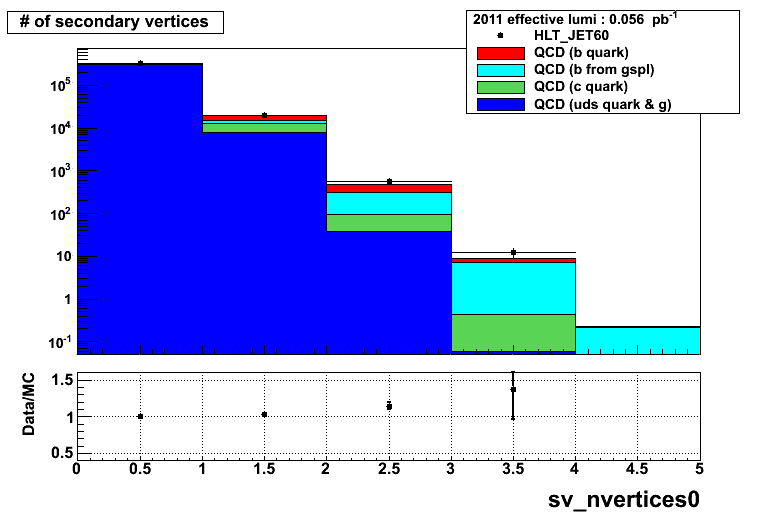
\includegraphics[width=0.32\textwidth]{figures/sv_nvertices0_Log.png}
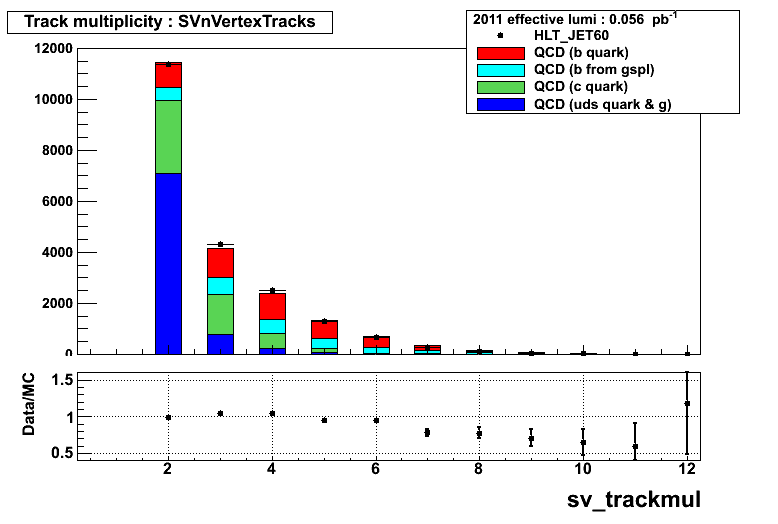
\includegraphics[width=0.32\textwidth]{figures/sv_trackmul_Linear.png}
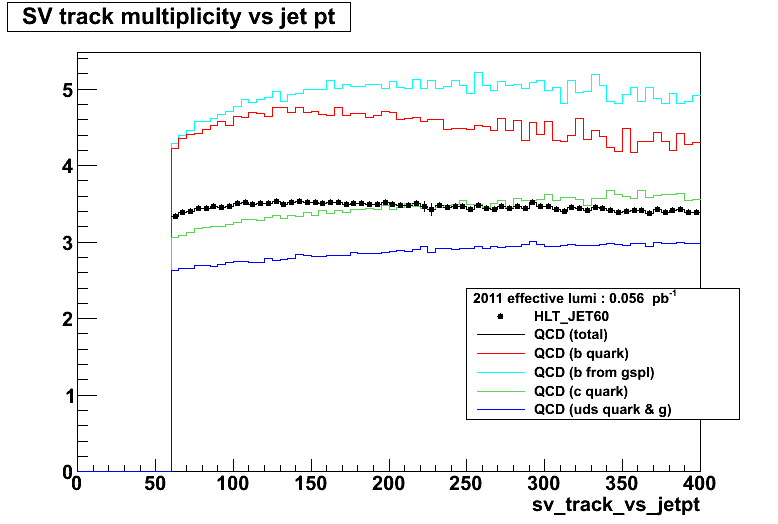
\includegraphics[width=0.32\textwidth]{figures/sv_track_vs_jetpt_Linear.png}
\caption{Left: number of reconstructed secondary vertices per jet, middle: number of tracks at the reconstructed secondary vertex, right: average number of tracks at the secondary vertex versus jet $p_t$. }
\label{fig:vertexNtracks}
\end{figure}

\begin{figure}[h!]
\centering
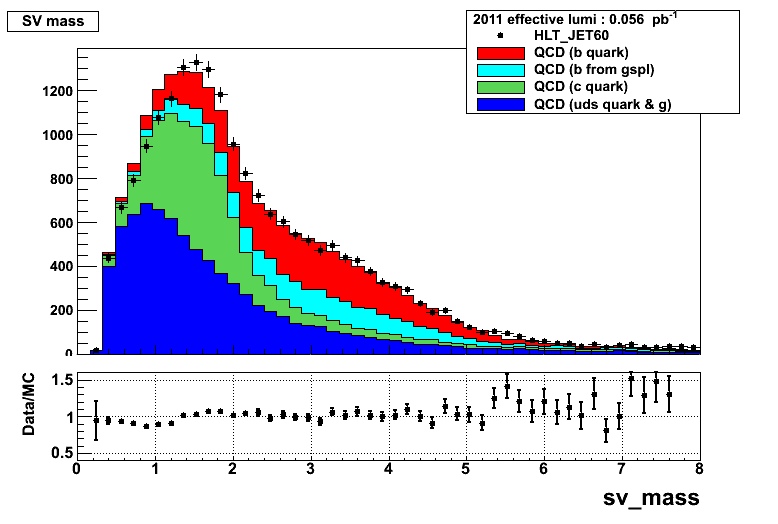
\includegraphics[width=0.32\textwidth]{figures/sv_mass_Linear.png}
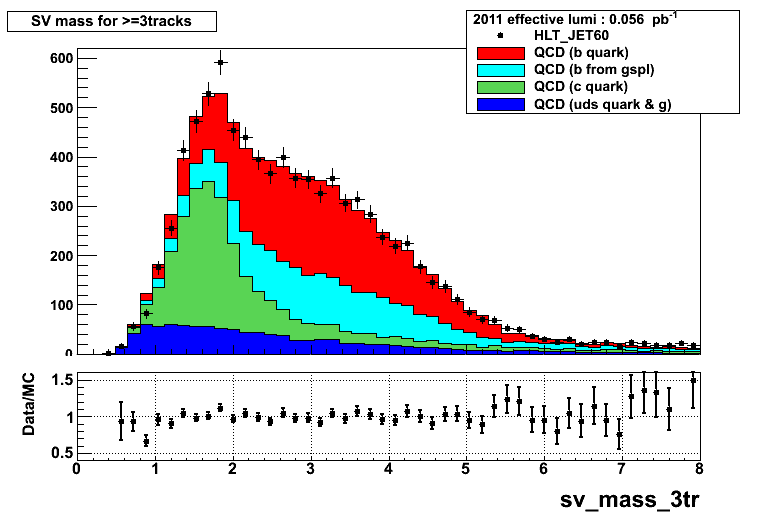
\includegraphics[width=0.32\textwidth]{figures/sv_mass_3tr_Linear.png}
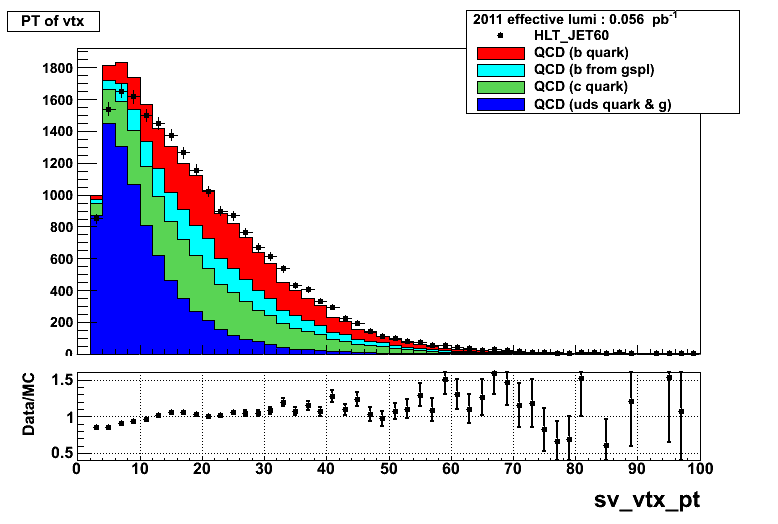
\includegraphics[width=0.32\textwidth]{figures/sv_vtx_pt_Linear.png}
\caption{Left: vertex mass with two or more reconstructed tracks at the vertex. Middle: vertex mass with three or more tracks at the vertex. Right: transverse momentum of the secondary vertex (with two or more tracks). }
\label{fig:vertexMass}
\end{figure}


An important quantity which is sensitive to the lifetime of B hadron decays is the  distance between primary and secondary vertex. As for the impact paramter, the significance of this quantity is used in b-tagging algorithms. Figure \ref{fig:vertexdistance} shows the flight distance significance, the normalized $\chi^2$ of the vertex fit and the energy ratio of tracks at the secondary vertex with respect to all tracks in the jet.

\begin{figure}[h!]
\centering
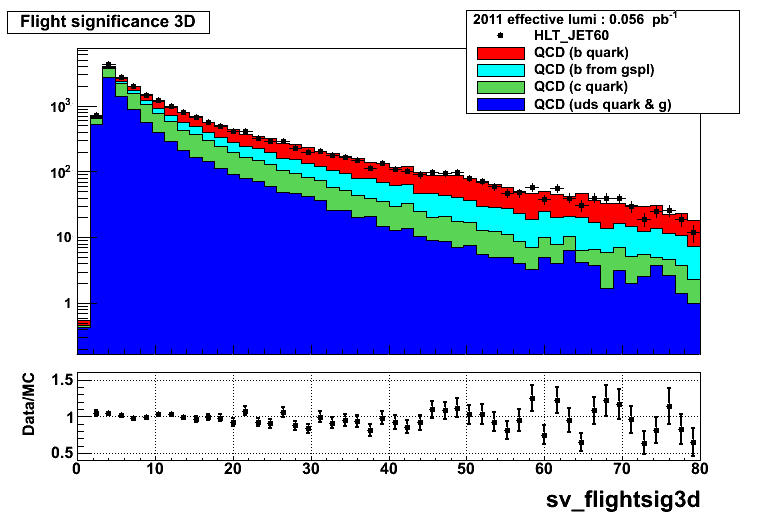
\includegraphics[width=0.32\textwidth]{figures/sv_flightsig3d_Log.png}
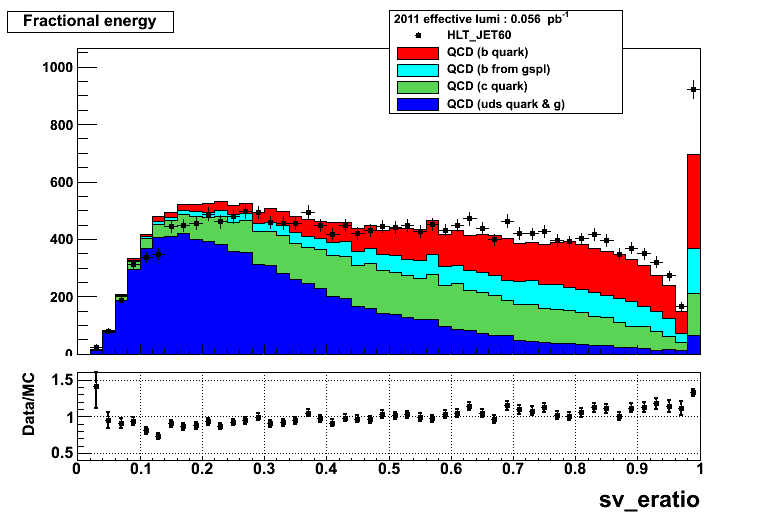
\includegraphics[width=0.32\textwidth]{figures/sv_eratio_Linear.png}
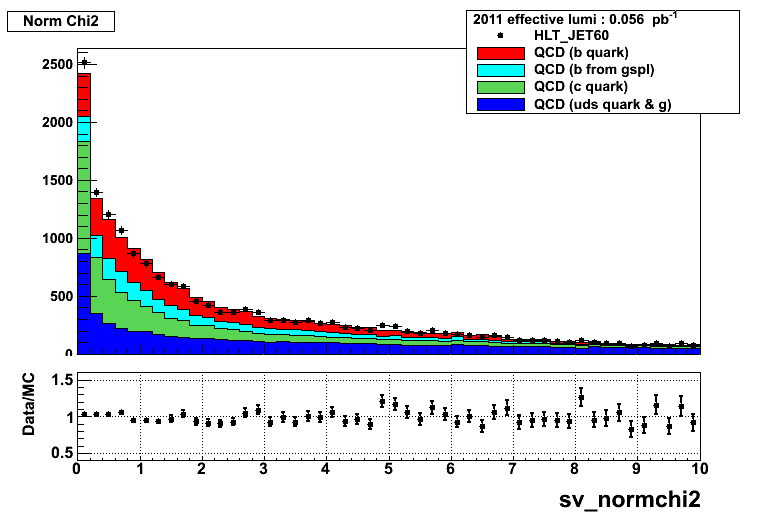
\includegraphics[width=0.32\textwidth]{figures/sv_normchi2_Linear.png}
\caption{Left: vertex flight distance significance. Middle: ratio of track energy at the secondary vertex with respect to all selected tracks in the jet. Right: vertex fit normalized $\chi^2$. }
\label{fig:vertexdistance}
\end{figure}

Two different directions can be defined at the secondary vertex: the flight direction, which points from the primary vertex to the secondary vertex and the direction of the vertex momentum which is the sum of all vertex track momenta. The angle between these two directions measured in $\Delta R$ as well as the angle with the jet axis are shown in Figure~\ref{fig:vertexAngles}.

\begin{figure}[h!]
\centering
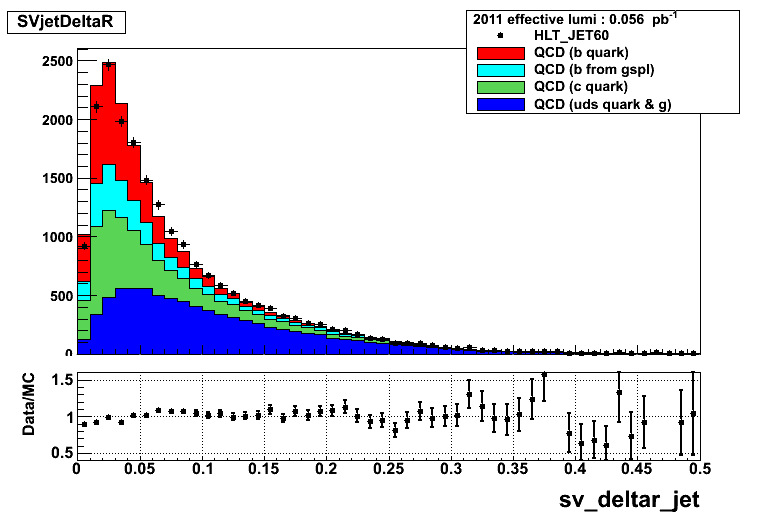
\includegraphics[width=0.32\textwidth]{figures/sv_deltar_jet_Linear.png}
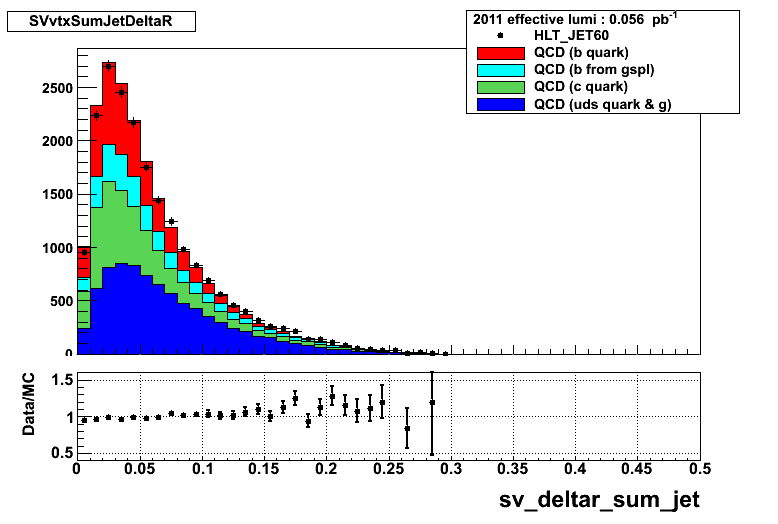
\includegraphics[width=0.32\textwidth]{figures/sv_deltar_sum_jet_Linear.png}
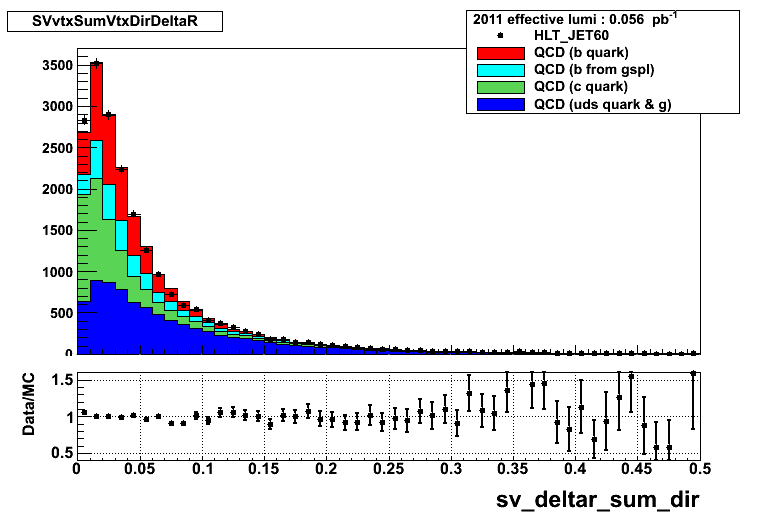
\includegraphics[width=0.32\textwidth]{figures/sv_deltar_sum_dir_Linear.png}
\caption{Left: angular distance in $\Delta R$ between jet axis and vertex direction. Middle: angular distance in $\Delta R$ between jet axis and the sum of track momenta at the vertex, Right: angular distance in $\Delta R$ between vertex direction and the sum of track momenta at the vertex. }
\label{fig:vertexAngles}
\end{figure}